\documentclass[../main.tex]{subfiles}
\graphicspath{
    {"../img/"}
    {"img/"}
}
\begin{document}

\textbf{Z poprzedniego wykładu:}
\begin{align*}
    f(x_0+h) &= f(x_0) + \sum_{i=1}^n \frac{\partial f}{\partial x^i} (x_0) h^i + \frac{1}{2!}\sum_{\substack{i=1\\ j=1}}^n \frac{\partial^2 f}{\partial x^i \partial x^j} (x_0) h^i h^j  + \dots +  \\
&+ \frac{1}{p!} \sum_{\substack{i_1 = 1\\ \vdots \\ i_p = 1}}^n \frac{\partial^p f}{\partial x^{i_1} \dots \partial x^{i_p+1}} (x_0) h^{i_1} \dots h^{i_p} + R_{p+1} (x_0, h),
\end{align*}
gdzie reszta wygląda tak:
\[
    R_{p+1} (h) = \frac{1}{(p+1)!} \sum_{\substack{i_1 = 1\\ \dots \\i_{p+1} = 1}}^n \frac{\partial^{p+1} f}{\partial x^{i_1} \dots \partial x^{i_p+1}} \underset{\substack{0<\theta<1\\ \text{ wersja } \mathbb{R}^n \text{ dla }\\"x_0 < c < x_0 +h"}}{(x_0+\theta h)} h^{i_1} \dots h^{i_{p+1}}.
\]

\begin{obserwacja}(bardzo ważna zależność!)\\
    \[
        \lim\limits_{h \to 0}\frac{R_{p+1} (x_0,h)}{||h||^p} \to 0.
    \]
\end{obserwacja}

\begin{przyklad}
$f: \mathbb{R}^2 \to \mathbb{R}, \quad f(x,y) = x^2y^3, f'(x,y) = \Big [ 2xy^3, 3x^2y^2 \Big ]$.

Jeżeli $h = \left [ \begin{matrix}
h_1\\
h_2\\
 \end{matrix}\right ]$, to wtedy

\begin{align*}
\sum_{\substack{i=1 \\ j=1}}^2 \frac{\partial^2 f}{\partial x^i \partial x^j} h^i h^j
&=\frac{\partial^2 f}{\partial x^1 \partial x^1} h^1 h^1 + \frac{\partial^2 f}{\partial x^1 \partial x^2} h^1 h^2 + \frac{\partial^2 f}{\partial x^2 \partial x^1} h^2 h^1 + \frac{\partial^2 f}{\partial x^2 \partial x^2} h^2 h^2 =\\
&= \Big [ h_1, h_1 \Big ] \left [ \begin{matrix}
\frac{\partial^2 f}{\partial x_1^2}  &\frac{\partial^2 f}{\partial x_1 \partial x_2} \\
\frac{\partial^2 f}{\partial x_2 \partial x_1}  &\frac{\partial^2 f}{\partial x_2^2}  \end{matrix}\right ] \left [ \begin{matrix}
h_1\\
h_2 \end{matrix}\right ]
\end{align*}
    \textbf{To czy ta macierz jest uśmiechnięta etc. (dodatnio/ujemnie określona) na algebrze.}

\end{przyklad}

\pagebreak
\subsection{Minima i maksima}
\textbf{Przypomnienie:}
Niech $f: \mathcal{O}\to \mathbb{R}, \mathcal{O}\subset \mathbb{R}^n, \mathcal{O}$ - otwarty, $x_0 \in \mathcal{O}$\\
Mówimy, że $f$ ma w $x_0$ minimum lokalne, jeżeli:
\[
    \underset{\eta > 0}{\exists} \quad
\underset{\substack{
x\in K(x_0,\eta)\\
K(x_0,\eta) \subset \mathcal{O}\\
x \neq x_0
}}{\forall} \quad f(x) > f(x_0), \underbrace{\left(f(x) < f(x_0)\right)}_{\text{albo maksimum}}.
\]

Albo inaczej:
\[
    \underset{\eta > 0}{\exists} \quad\underset{h}{\forall}\quad ||h|| < \eta, \quad x_0+h \in \mathcal{O}, h \neq 0\text{, to wtedy } f(x_0+h)>f(x_0).
\]

\begin{figure}[h]
    \centering
    \includegraphics[width=0.5\textwidth]{fig_12}
    \caption{istnieje otoczenie, dla którego  $f(x)>f(x_0)$ (nie musi być styczne!)}
\end{figure}

\begin{stw}
jeżeli $f: \mathcal{O} \rightarrow \mathbb{R}, \mathcal{O}$ - otwarty, $x_0 \in \mathcal{O}, f$ - posiada w $x_0$ minimum lub maksimum lokalne, to $$\frac{\partial f}{\partial x^i} (x_0) = 0, i = 1,\dots,n$$
działa tylko w prawo, bo możliwe są punkty przegięcia (siodła)
\end{stw}

\textbf{Uwaga:} jeżeli $f: U\to \mathbb{R}$ i $U$ - domknięta, to należy zbadać zachowanie funkcji osobno na $int(U)$ oraz na $U - \{int(U)\}$

\begin{proof}

Niech $g_h (t) = f(x_0+th) \text{ i } g: [0,\epsilon [ \to \mathbb{R}$.\\
Zauważmy, że jeżeli $f$ ma minimum lub maksimum w $x_0$, to znaczy, że $g_h (t)$ ma minimum lub maksimum w $t = 0$, czyli
\[
    \left . \frac{\partial}{\partial t} g_h(t) \right |_{t=0} = 0,
\]

czyli dla $x_0 = \big ( x_0^1, x_0^2, \dots, x_0^n),\quad h = \big ( h^1, h^2, \dots, h^n)$

\begin{align*}
    \left . \frac{d}{dt} g_h (t) \right |_{t=0} &= \left .\frac{d}{dt} f(x_0^1 + th^1, \dots, x_0^n + th^n) \right |_{t=0} = \\
&= \frac{\partial f}{\partial x^1} (x_0 + th^1) h^1 + \frac{\partial f}{\partial x^2} (x_0 + th^2) h^2 + \dots + \left .\frac{\partial f}{\partial x^n} (x_0 + th^n) \right |_{t=0}=\\
&=\sum_{i=1}^n \frac{\partial f}{\partial x^i} (x_0) h^i = 0 \quad |\underset{h}{\forall}: ||h|| < \eta
,\end{align*}
to znaczy:
\[
    \frac{\partial f}{\partial x^i} (x_0) = 0,\quad i = 1,\dots,n.
\]
\end{proof}
\textbf{Uwaga: } jest to warunek konieczny, a nie dostateczny!

\pagebreak
\begin{tw}
Niech
\begin{align*}
    &f: \mathcal{O} \to \mathbb{R},\\
    &\mathcal{O}\subset\mathbb{R}^n,\\
    &x_0\in\mathcal{O}, \quad \mathcal{O} \text{ - otwarty},\\
    &f \in C^{2p} (\mathcal{O}),\\
    &f'(x_0) = 0, f''(x_0) = 0,\dots,f^{(2p-1)} (x_0) = 0
.\end{align*}
oraz spełniony jest warunek
    \[
        \underset{c > 0}{\exists} \quad\underset{\eta > 0}{\exists} \quad\underset{h\in K(x_0,\eta)}{\forall}: \quad \sum_{\substack{i_1 = 1\\ \vdots \\ i_{2p} = 1}}^n \frac{\partial^{(2p)} f}{\partial x^{i_1} \dots \partial x^{i_{2p}}} (x_0) h^{i_1} \dots h^{i_{2p}} \geq c ||h||^{2p} (\leq c||h||^{2p})
    \]
to wtedy $f$ ma w $x_0$ minimum (maksimum) lokalne.
\end{tw}

\begin{proof}
(wersja uproszczona dla minimum i dla $f$ klasy $C^{2p+1}(\mathcal{O}))$.\\
Jeżeli $f$ spełnia założenie z twierdzenia, to wtedy
\begin{equation}
    \label{eq: eq_5.1}
    f(x_0+h)-f(x_0) = \underbrace{\frac{1}{(2p)!} \sum_{i_1 = 1\ldots i_{2p} = 1}^{2p} \frac{\partial^{(2p)} f(x_0)}{\partial x^{i_1} \dots x^{i_{(2p)}}} h^{i_1} \dots h^{i_{(2p)}}}_{(*)} + r_{2p + 1} (x_0 + h)
\end{equation}
Wiemy też , że
    \[
        \underset{c > 0}{\exists}\quad \underset{\eta > 0}{\exists} \underset{\substack{\text{Chodzi o to, żeby reszta}\\ \text{ nie mogła tego przekroczyć}}}{\quad(\ref{eq: eq_5.1})(*)) \geq c ||h||^{2p}}
    .\]
Chcemy pokazać, że
    \[
        \underset{\eta}{\exists} \quad \underset{||h||<\eta}{\forall} \Big | r_{2p+1} (x,h) \Big | \leq \underset{\substack{\text{albo 7,}\\ \text{albo 2019}}}{\frac{c}{2} ||h||^{2p}}
    .\]
Czyli chcemy zbadać wielkość:
    \[
        \frac{1}{(2p+1)!} \sum_{i_1 = 1 \ldots i_{2p+1} = 1}^n \underset{0 < \theta < 1}{\frac{\partial^{(2p+1)} f (x_0 + \theta h)}{\partial x^{i_1} \dots \partial x^{i_{(2p+1)}}}} h^{i_1} \dots h^{i_{(2p+1)}} = \left| \text{tu potrzebne założenie, że } f \in C^{2p+1} (\mathcal{O})\right| = r_{2p+1} (x,h)
    .\]
Zauważmy, że $\lim\limits_{h \to 0} \frac{r_{2p+1}(x_0, h)}{||h||^{2p}} \to 0$, ale zatem
    \[
        \underset{M>0}{\forall}\quad \underset{\eta}{\exists}\quad \underset{||h|| < \eta}{\forall} \frac{r_{2p+1}(x_0+h)}{||h||^{2p}} < M
    ,\]
czyli
\[
    \left| \frac{r_{2p+1} (x_0,h)}{||h||^{2p}} \right| < M.
\]
    \[
        \underset{M}{\forall}\quad \underset{\eta}{\exists}\quad \underset{||h|| < \eta}{\forall}\quad \Big | r_{2p+1} (x_0,h) \Big | < M \big | \big |h \big | \big |^{2p}
    \]
czyli jak przyjmiemy $M = \frac{c}{2}$ to dostajemy
    \[
        \underset{\eta}{\exists}\quad \underset{||h||<\eta}{\forall}\quad f(x_0+h)-f(x_0) \geq \frac{c}{2} ||h||^{2p}
    \]
\end{proof}

\textbf{Uwaga:} dlaczego warunek $( - \big| - ) > c ||h||^{2p}$, a nie po prostu $( - \big| - ) > 0$?

\begin{przyklad}

    \[
        f(x,y) = x^2 + y^4,\quad \frac{\partial f}{\partial x} = 2x,\quad \frac{\partial f}{\partial y} = 4y^3
    .\]
\[
    f'() = 0 \iff (x,y) = (0,0)
\]
Badamy: $f(0+h) - f(0) = \big [ h_1, h_2 \big ] \left [ \begin{matrix}
2 &0\\
0 &2y^2\\
\end{matrix}\right ]
\left [ \begin{matrix}
h_1\\
h_2\\\end{matrix}\right ]
= \big [ h_1, h_2 \big ] \left [ \begin{matrix}
2 &0\\
0 &0\\ \end{matrix}\right ]
\left [ \begin{matrix} h_1\\
h_2\end{matrix}\right ] = 2h_1^2$
Czyli $f(0+h) - f(0) \star  2h_1^2$ - minimum? maksimum? - zależy w którą stronę.\\
$h = \left [ \begin{matrix}
h_1\\
0\\
\end{matrix}\right ] $ - minimum,
$h = \left [ \begin{matrix}
0\\
h_2\\
\end{matrix}\right ] $ - równo,
coś takiego - punkt siodłowy.\\
Widzimy zatem, że nie jest spełniony warunek
\[
    \underset{c}{\exists}\left[ h_1, h_2 \right ] \left[ \begin{matrix}
2 &0\\
0 &0\\
\end{matrix}\right ]
\left [ \begin{matrix}
h_1\\
h_2\\
    \end{matrix}\right ] \geq c \left\Vert h \right\Vert ^2
,\]
bo dla
\[
    h = \left [ \begin{matrix}
0\\
h_2\\
    \end{matrix}\right ] \quad 0 \not\geq c \left\Vert \left [ \begin{matrix}
0\\
h_2\\
\end{matrix}\right ] \right\Vert
\]
\end{przyklad}

\subsection{Kilka fajnych zastosowań}
\[
    \frac{mv^2}{2} =
\left [ \begin{matrix}
 &v &\\ \end{matrix}\right ]
\left [ \begin{matrix}
    \frac{m}{2}\\
&\frac{m}{2}\\
   & & \ddots\\
    \end{matrix}\right ]  \left [ \begin{matrix}
\\
v\\
 \\\end{matrix}\right ]
\]
\[
    \frac{I \omega^2}{2} =
    \left [ \begin{matrix}
    &\omega &
    \\ \end{matrix}\right ]
    \left [ \begin{matrix}
    \frac{I}{2} & &\\
     &\frac{I}{2} &\\
     & &\ddots\\
     \end{matrix}\right ] \left [ \begin{matrix}
    \\
    \omega\\
    \\
    \end{matrix}\right ]
\]

\end{document}
